\slide{dsniff - dataafl�sning}

\begin{list1}
\item en sniffer til mange usikre protokoller
\item inkluderer {\bfseries arpspoof}  
\item Lavet af Dug Song, dugsong@monkey.org
\item 
\begin{alltt}
\small
dsniff  is  a  password sniffer which handles FTP, Telnet,
SMTP, HTTP, POP, poppass, NNTP, IMAP, SNMP, LDAP,  Rlogin,
RIP,  OSPF,  PPTP  MS-CHAP, NFS, VRRP, YP/NIS, SOCKS, X11,
CVS, IRC, AIM, ICQ, Napster,  PostgreSQL,  Meeting  Maker,
Citrix  ICA,  Symantec  pcAnywhere, NAI Sniffer, Microsoft
SMB, Oracle SQL*Net, Sybase and Microsoft SQL protocols.
\end{alltt}
\end{list1}

\slide{dsniff foruds�tninger}

\begin{center}
  \colorbox{white}{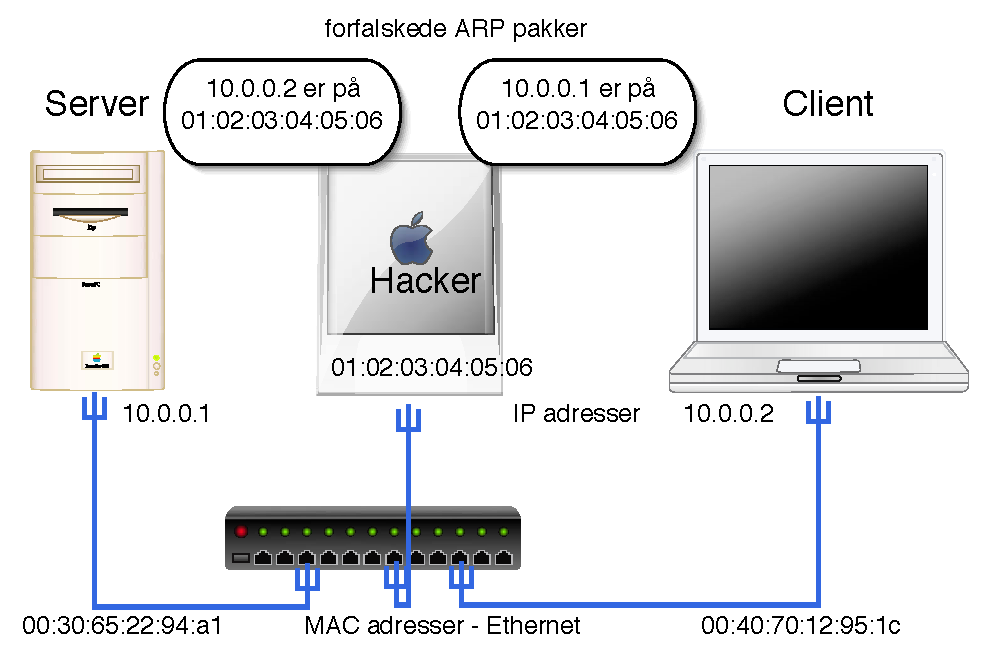
\includegraphics[width=12cm]{images/arp-spoof.pdf}}  
\end{center}

\begin{list1}
\item Afl�sning af hemmeligheder - kodeord m.v.
\item Hvilke foruds�tninger er der for at bruge Dsniff?
\item dsniff skal have adgang til trafikken ...
%\item P� et system med dsniff installeret findes manual siderne
%  {\bfseries man arpspoof} og {\bfseries man dsniff}
\end{list1}


%%% Local Variables: 
%%% mode: latex
%%% TeX-master: "tcpip-security"
%%% End: 
